\documentclass[tikz]{standalone}
\usepackage{mathtools}
\usepackage{etoolbox}
\usetikzlibrary{intersections}

\newcommand{\drawcsys}[5][0]{
    \def\vstep{#1}
    \def\vxmin{#2}
    \def\vxmax{#3}
    \def\vymin{#4}
    \def\vymax{#5}

	\ifstrequal{#1}{0}{}{%
        \draw[help lines,step=\vstep] (\vxmin,\vymin) grid (\vxmax,\vymax);
    }
    \draw[->,thick] (\vxmin,0) -- (\vxmax,0) node[anchor=north] {$x$};
    \draw[->,thick] (0,\vymin) -- (0,\vymax) node[anchor=east]  {$y$};
}


\begin{document}
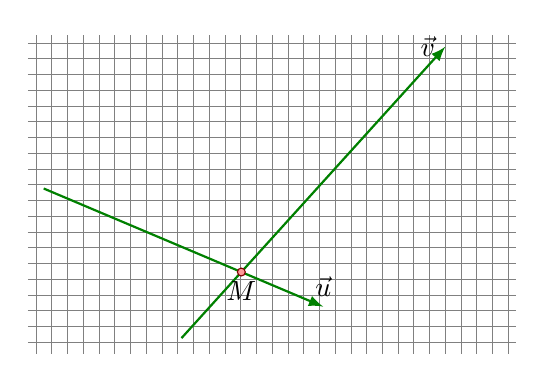
\begin{tikzpicture}[vector/.style={thick,-latex,green!50!black}]
    \draw[ultra thin,help lines,step=.2] (-.5,-.55) grid (5.7,3.5);
	\draw[help lines,step=1] (-.5,-.55) grid (5.7,3.5);

	\draw[name path=vecu] [vector] (-.3,1.55) -- (3.25,.05) node [black,above] {$\vec u$};
	\draw[name path=vecv] [vector] (1.45,-.35) -- (4.8,3.35) node [black,left] {$\vec v$};

	\path[name intersections={of=vecu and vecv}];
	\coordinate [label=270:$M$](M) at (intersection-1);
	\filldraw[draw=red!50!black,fill=red!40!white] (M) circle[radius=.05];
\end{tikzpicture}
\end{document}
